\section*{\large{ВВЕДЕНИЕ}}

Цель лабораторной работы --- разработать программу шифровальной машины <<RSA>> \cite{Enigma}.

Задачи лабораторной работы:

\begin{enumerate}
    \item провести анализ работы шифровальной машина <<RSA>>;
    \item описать алгоритм шифрования;
    \item релизовать описанный алгоритм.
\end{enumerate}

\clearpage
\section{Аналитическая часть}

\subsection{Алгоритм шифрования RSA}

\textbf{RSA} \cite{Enigma} ---  криптографический алгоритм с открытым ключом, основывающийся на вычислительной сложности задачи факторизации.

\textbf{Алгоритм}:

\begin{itemize}
	\item[---] Выбираем два случайных простых числа p и q.
	\item[---] Вычисляем их произведение: N = p * q.
	\item[---] Вычисляем функцию Эйлера: $\varphi(N) = (p-1) * (q-1)$.
	\item[---] Выбираем число e (обычно простое, но необязательно), которое меньше $\varphi(N)$ и является взаимно простым с $\varphi(N)$ (не имеющих общих делителей друг с другом, кроме 1).
	\item[---] Ищем число d, обратное числу e по модулю $\varphi(N)$ .Т.е. остаток от деления (d*e) и $\varphi(N)$ должен быть равен 1. Найти его можно через расширенный алгоритм Евклида.

\end{itemize}

Алгоритм шифрования RSA может использоваться в следующих режимах.

\begin{enumerate}
	\item[1.] \textbf{MD5}  --- 128-битный алгоритм хеширования, разработанный профессором Рональдом Л. Ривестом из Массачусетского технологического института (Massachusetts Institute of Technology, MIT) в 1991 году. Предназначен для создания «отпечатков» или дайджестов сообщения произвольной длины и последующей проверки их подлинности. Широко применялся для проверки целостности информации и хранения хешей паролей.
	\item[2.] \textbf{SHA1} --- алгоритм криптографического хеширования. Для входного сообщения произвольной длины  алгоритм генерирует 160-битное (20 байт) хеш-значение, называемое также дайджестом сообщения, которое обычно отображается как шестнадцатеричное число длиной в 40 цифр.
\end{enumerate}

\clearpage

\section{Конструкторская часть}

\subsection{Разработка алгоритма}

На рисунке \ref{fig:algo} представлена схема алгоритма шифрования RSA.

%

\begin{figure}[h!]
	\centering
	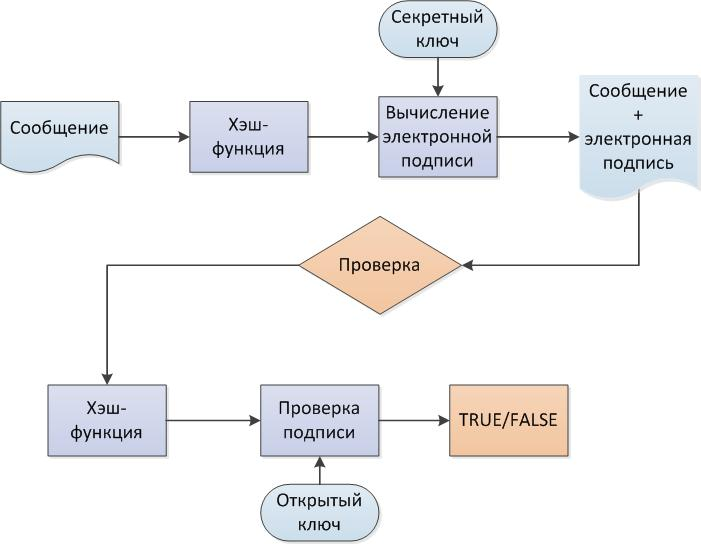
\includegraphics[width=\textwidth]{assets/images/RSA.jpeg}
	\caption{Схемы алгоритма RSA}
	\label{fig:algo}
\end{figure}
\clearpage

\section{Технологическая часть}

\subsection{Средства реализации}

Для реализации ПО был выбран язык C++ \cite{c++}.
В данном языке есть все требующиеся инструменты для данной лабораторной работы.
В качестве среды разработки была выбрана среда VS code \cite{vscode}.

\subsection{Реализация алгоритма}

Реализация OFB.

\begin{lstlisting}
    Keys calculateRSAKeys()
    {
      std::vector <largeIntegerType> primes(1034);
      std::ifstream fin("input/primes.txt");
      for(int i = 0; i < 1033; i++)
      {
        int temp;
        fin >> temp;
        primes[i] = temp;
      }
    
      largeIntegerType p = primes[rand() % 1033];
      largeIntegerType q = primes[rand() % 1033];
    
      largeIntegerType n = p * q;
    
      largeIntegerType functionE = (p - 1) * (q - 1);
    
      largeIntegerType e = 1;
      for (largeIntegerType i = functionE - 1; i > 0; --i)
      {
        if (gcd(i, functionE) == 1 && prime(i))
        {
          e = i;
          break;
        }
      }
    
      largeIntegerType d;
      for (largeIntegerType i = 0;; ++i)
      {
        if ((largeIntegerType)i * (largeIntegerType)e % (largeIntegerType)functionE == 1)
        {
          d = i;
          break;
        }
      }
    
      Keys keys{std::pair<largeIntegerType, largeIntegerType>{e, n}, std::pair<largeIntegerType, largeIntegerType>{d, n}};
      return keys;
    }
\end{lstlisting}


\subsection{Тестовые данные}

В таблице \ref{tbl:functional_test} приведены тесты для алгоритма шифрования RSA. 
Применена методология черного ящика. Тесты пройдены \textit{успешно}.

\begin{table}[ht!]
	\begin{center}
		\captionsetup{justification=raggedright,singlelinecheck=off}
		\caption{\label{tbl:functional_test} Функциональные тесты}
		\begin{tabular}{|c|c|c|}
			\hline
			Входная строка & Выходная строка \\ 
			\hline
			$ABOBA$ & $BCRGJ$\\
			$BCRGJ$  & $ABOBA$\\
			$<<>>$  & $<<>>$ \\
            $A$ & $T$\\
			$T$  & $A$\\
			\hline
		\end{tabular}
	\end{center}
\end{table}

\clearpage
\section*{\large{ЗАКЛЮЧЕНИЕ}}
В данной лабораторной работе:
\begin{enumerate}
    \item проведен анализ работы шифровальной машина <<RSA>>;
    \item описан алгоритм шифрования;
    \item реализован описанный алгоритм;
\end{enumerate}